% \section{Supplementary materials}
% \label{supp_mat}

% \setcounter{page}{1}
% \maketitlesupplementary


\renewcommand\thefigure{S\arabic{figure}}    
\setcounter{figure}{0}  
\renewcommand\theequation{S\arabic{equation}}    
\setcounter{equation}{0}
\renewcommand\thealgorithm{S\arabic{algorithm}}    
\setcounter{algorithm}{0}  
\renewcommand{\thesection}{\Alph{section}}
\renewcommand\thetable{S\arabic{table}}

\section{Shifting the latent code}\label{app:shift}
As described in Sec.~\ref{method}, we can shift an input image by shifting its extracted latent code. This requires inserting new columns/rows at the boundary of the noise maps. To guarantee that the inserted columns/rows are drawn from the same distribution as the rest of the noise map, we simply copy a contiguous chunk of columns/rows from a different part of the noise map. In all our experiments, we copied into the boundary the columns/rows indexed $\{50,\ldots,50+d-1\}$ for a shift of $d$ pixels. We found this strategy to work better than randomly drawing the missing columns/rows from a white normal distribution having the same mean and variance as the rest of the noise map. %In the case of having the latent space, as in generated images, we can also shift the latent space and insert random Gaussian noise in the blank pixels, however, this results in deviations from the original image.
Figure~\ref{fig:shifting_graph} depicts the MSE over the valid pixels that is incurred when shifting the noise maps. This analysis was done using 25 model-generated images. As can be seen, shifting our edit-friendly code results in minor degradation while shifting the native latent code leads to a complete loss of the image structure. 

\begin{figure}[H]
\centering
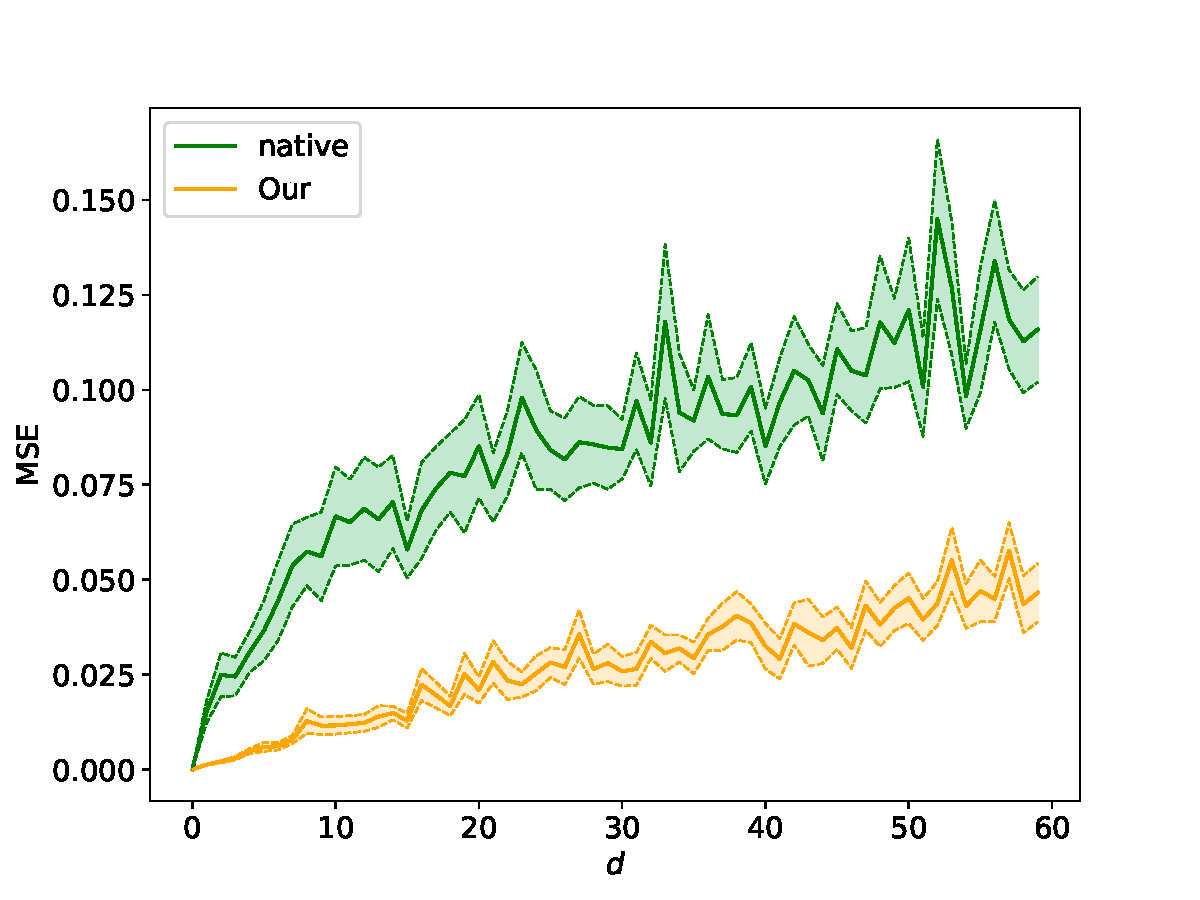
\includegraphics[width=0.5\textwidth]{ICCV23_submission/figures/mean-err-shifting.pdf}
\caption{\textbf{Shifting the latent code}. We plot the MSE over the valid pixels after shifting the latent code and generating the image. The colored regions represent one standard error of the mean (SEM) in each direction.}
\label{fig:shifting_graph}
\end{figure}

\clearpage

\section{The effect of the numerical error} 
In Algorithm~\ref{alg:example} we add a correction step for avoiding numerical drifting. This step assists in achieving perfect reconstruction. Note that in order to reconstruct the input image, the hyper-parameters used to extract the noise maps should be identical to the ones used for sampling. Specifically, the prompt, $T_{\text{skip}}$, and strength parameters should be the same in the function $\mu_t(x_t)$ used for the inversion (Eq.~\ref{eq:z_t}) and in the function $\mu_t(x_t)$ used during sampling (Eq.~\ref{eq:diffusion}). We note that the effect of the numerical drifting is noticeable only when using a large strength parameter (see second and third column in Fig.~\ref{fig:reconstruction_for_rebuttal}). By default, when performing text-based editing, we do not use extreme values for the strength parameter, and therefore in such cases this correction is not needed (rightmost column in Fig.~\ref{fig:reconstruction_for_rebuttal}).


We calculate the PSNR between the images with and without the correction for the example that appears in Fig.~\ref{fig:reconstruction_for_rebuttal}. In the reconstruction case, using $\text{strength}=30$, the PSNR can drop to below 17dB. As noted, this correction is not needed for editing, where the PSNR between the edited images with and without the correction is 67.4dB.

\begin{figure}[H]
\centering
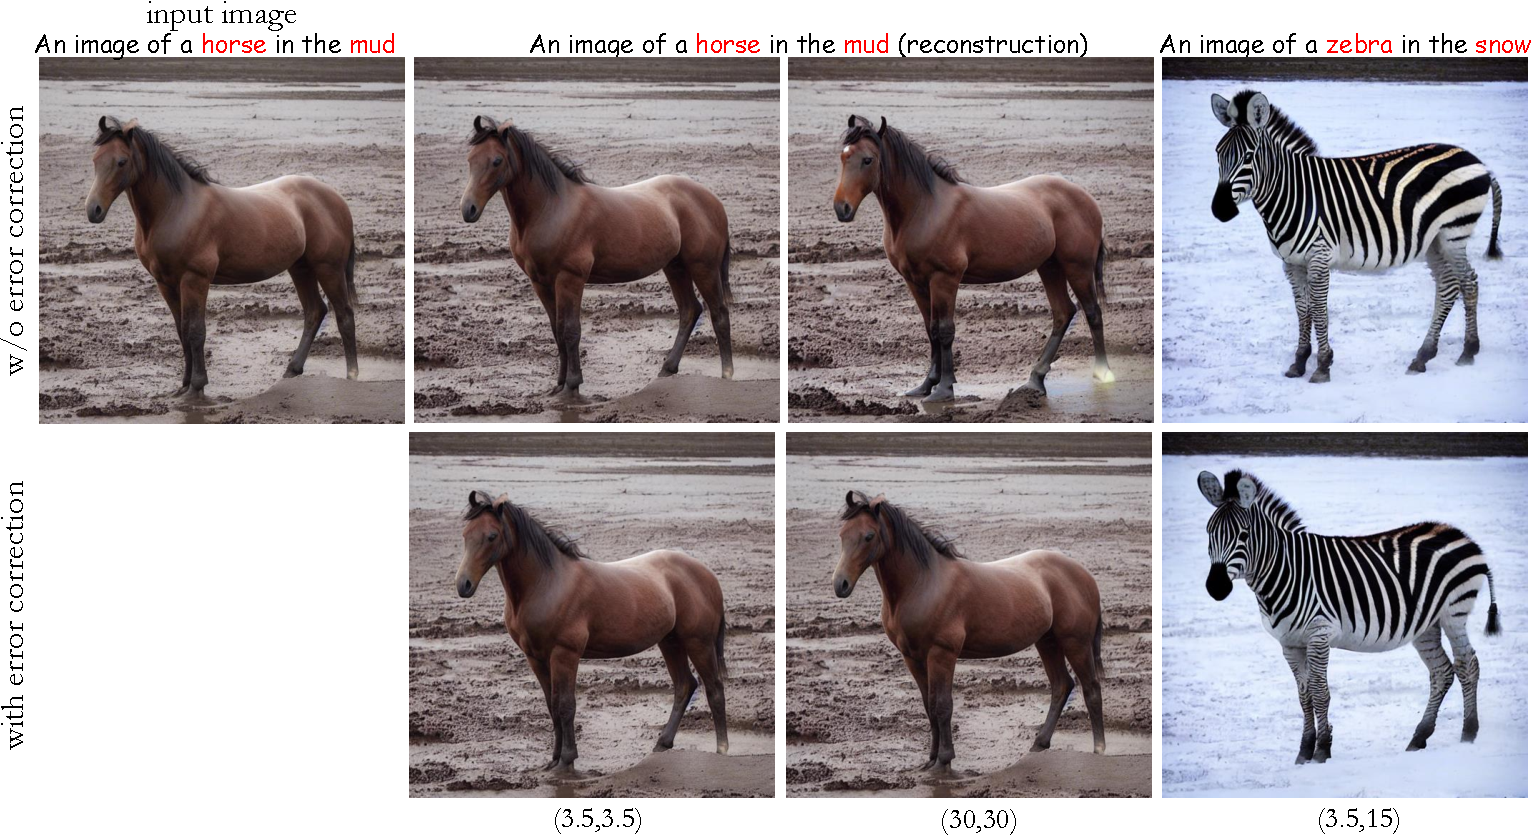
\includegraphics[width=\columnwidth]{ICCV23_submission/figures/reconstruction_for_rebuttal.pdf}
\caption{\textbf{Error correction effect.} 
Below the images, we specify the strength parameters used for the inversion (first number within the parentheses) and the sampling (second number within the parentheses). Above the images, we specify the prompt used. Above the leftmost column is $p_{\text{src}}$, while above the other columns is $p_{\text{tar}}$. The parameter $T_{\text{skip}}$ is set to 36, as in our experiments in the main text. The second and third columns show reconstructions. As can be seen, with a large strength parameter, the reconstruction is not perfect without the correction (\eg the head and the leg of the horse). However, this numerical drifting does not influence the editing quality (rightmost column).}

\label{fig:reconstruction_for_rebuttal}
\end{figure}




\clearpage

\section{CycleDiffusion}
As mentioned in Sec.~\ref{sec:properties}, CycleDiffusion~\cite{Wu22} extracts a sequence of noise maps $\{x_T,z_T,\ldots,z_1\}$ for the DDPM scheme. However, in contrast to our method, their noise maps have statistical properties that resemble those of regular sampling. %\paragraph{Noise map properties}
%The joint distribution of these maps is close to that used in regular sampling, i.e., standard Gaussian noise. Hence, we claim that these noise maps are not suitable for editing images. 
This is illustrated in Fig.~\ref{fig:statistics_images_CycleDiffusion}, which depicts the per-pixel standard deviations of $\{z_t\}$ and the correlation between $z_t$ and $z_{t-1}$ for CycleDiffusion, for regular sampling, and for our approach. These statistics were calculated over 10 images using an unconditional diffusion model trained on Imagenet, with $\eta=1.0$, $\text{strength}=3$ and $T_{\text{skip}} = 30$ as hyper parameters.
As can be seen, the CycleDiffusion curves are almost identical to those of regular sampling, and are different from ours. 

\begin{figure}[H]
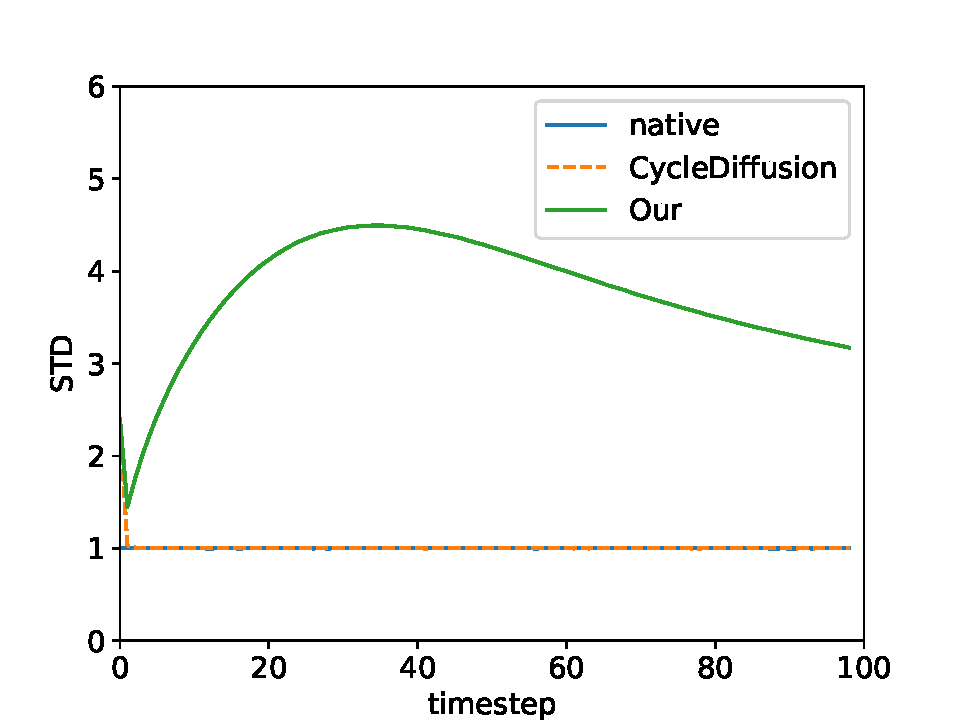
\includegraphics[width=0.485\textwidth, trim={0.8cm 0cm 1.2cm 0cm},clip]{ICCV23_submission/figures/std_with_cycle_native.pdf}
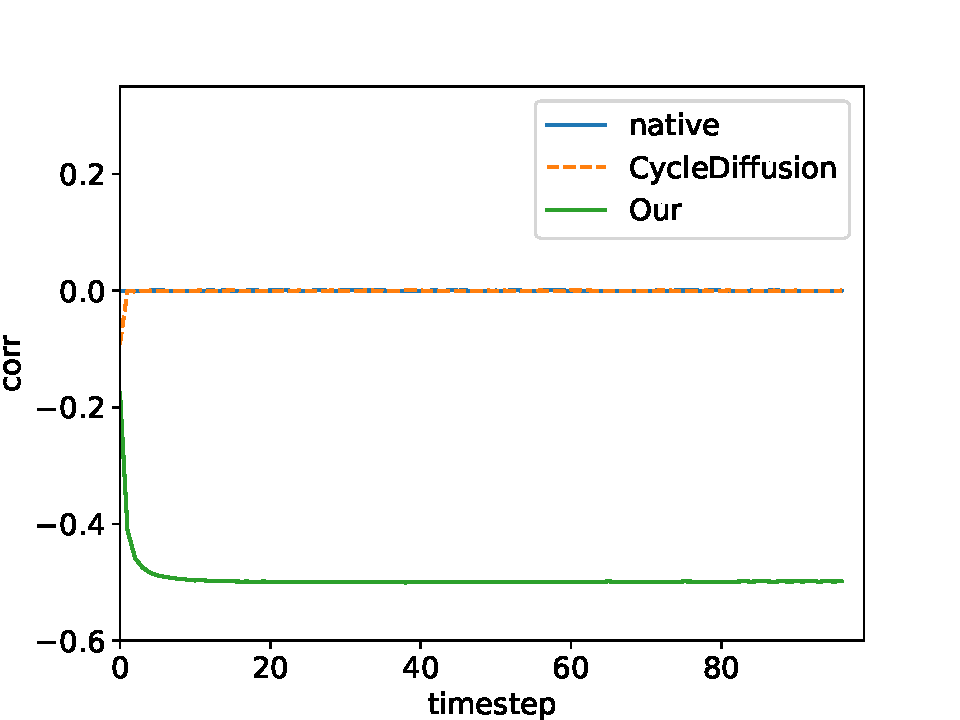
\includegraphics[width=0.515\textwidth, trim={0cm 0cm 1.2cm 0cm},clip]{ICCV23_submission/figures/corr_with_cycle_native.pdf}
\caption{\textbf{CycleDiffusion noise statistics.} Here we show the per-pixel standard deviations of $\{z_t\}$ and the per-pixel correlation between them for mssodel-generated images.}
\label{fig:statistics_images_CycleDiffusion}
\end{figure}

\vspace{-4.cm}
The implication of this is that similarly to the native latent space, simple manipulations on CycleDiffusion's noise maps cannot be used to obtain artifact-free effects in pixel space. This is illustrated in Fig.~\ref{fig:flip_shift_CycleDiffusion} in the context of horizontal flip and horizontal shift by 30 pixels to the right. As opposed to Cycle diffusion, applying those transformations on our latent code, leads to the desired effects, while better preserving structure.% preserves the structure operations of real images using the latent space extracted by CycleDiffusion. 

\vspace{-0.2cm}
This behavior also affects the text based editing capabilities of CycleDiffusion. In particular, the CLIP similarity and LPIPS distance achieved by CycleDiffusion on the modified ImageNet-R-TI2I dataset are plotted in Fig.~\ref{fig:clip_lpips}. As can be seen, when tuned to achieve a high CLIP-similarity (\ie to better conform with the text), CycleDiffusion's LPIPS loss increases significantly, indicating that the output images become less similar to the input images. For the same level of CLIP similarity, our approach achieves a substantially lower LPIPS distance.

\begin{figure}[H]
\centering
\includegraphics[width=0.75\textwidth]{ICCV23_submission/figures/cycleDiffusion-flip-and-shift.pdf}
\caption{\textbf{Flip and shift with CycleDiffusion and with our inversion.}}
\label{fig:flip_shift_CycleDiffusion}
\end{figure}



%\paragraph{Quantitative evaluation}


\clearpage

% \section{The effect of hyper-parameters}
\section{The effect of skip and strength parameters}\label{app:SkipAndStrength}
Recall from Sec.~\ref{sec:text-guided} that in order to perform text-guided image editing using our inversion, we start by extracting the latent noise maps while injecting the source text into the model, and then generate an image by fixing the noise maps and injecting a target text prompt. Two important parameters in this process are  $T_{\text{skip}}$, which controls the timestep ($T-T_{\text{skip}}$) from which we start the generation process, and the strength parameter of the classifier-free scale~\cite{Ho21}.  Figure~\ref{fig:skip_strength} shows the effects of these parameters. When $T_{\text{skip}}$ is large, we start the process with a less noisy image and thus the output image remains close to the input image. On the other hand, the strength parameter controls the compliance of the output image with the target prompt.

\begin{figure*}[h]
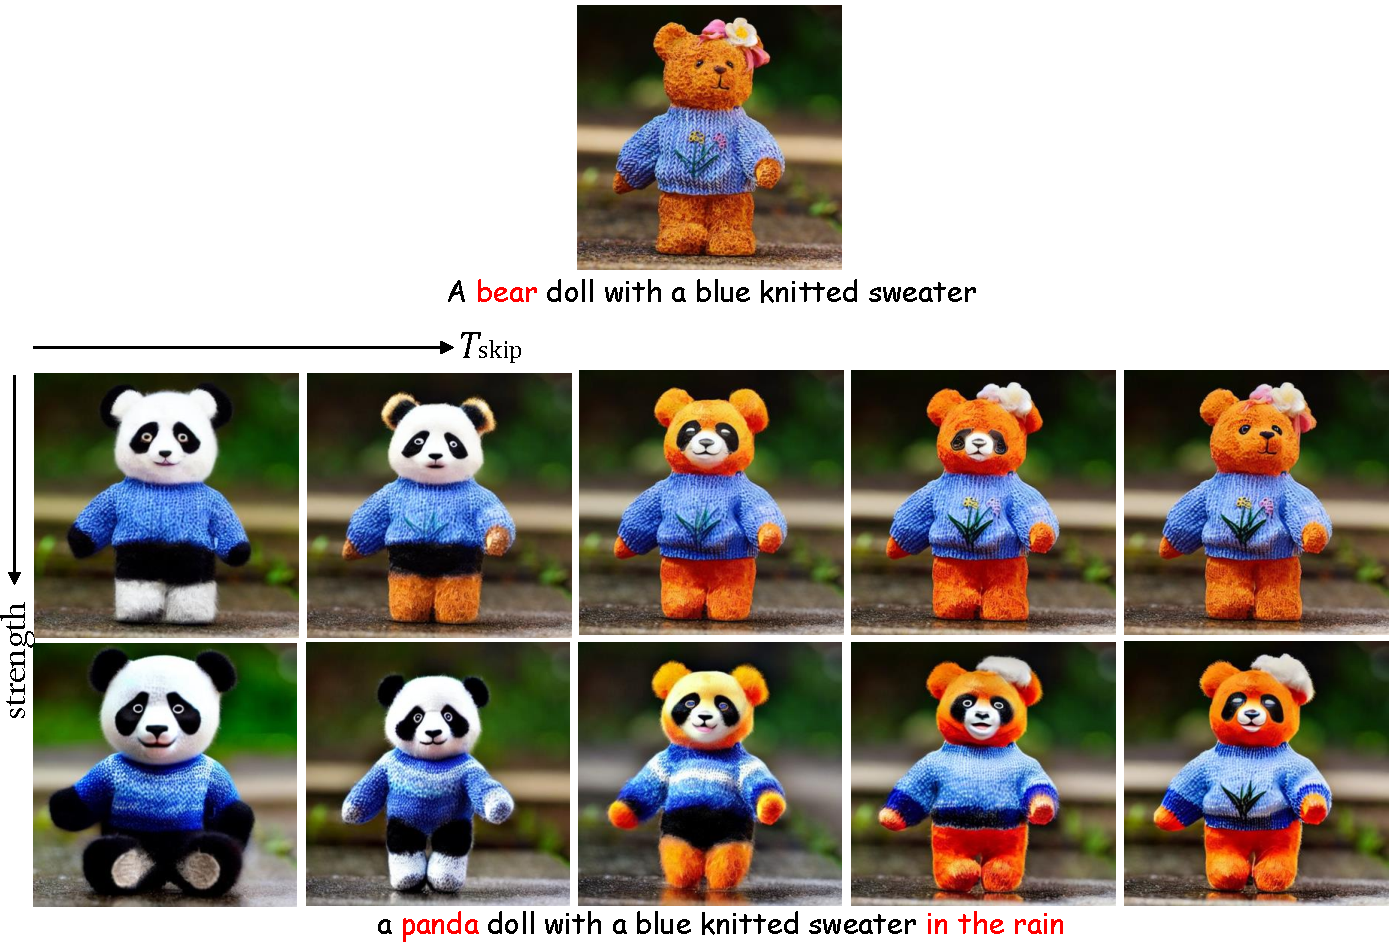
\includegraphics[width=\textwidth]{ICCV23_submission/figures/skip_sclae_balance.pdf}
\caption{\textbf{The effects of the skip and the strength parameters}.}
\label{fig:skip_strength}
\end{figure*}

% \subsection{Diffusion step number}
% \label{app:DiffusionStepNumber}
% Below we test the effect of the diffusion number steps over the CLIP and LPIPS score. We compare the methods over the ImageNet-R-TI2I dataset with $20,50$ and $200$, in addition to $100$ steps we report in Sec.~\ref{sec:evalution}. In this test we did not change the strength parameter but only the $T_{\text{skip}}$ parameter to be consistent with the value number of steps (i.e., if at 100 steps our $T_{\text{skip}}=36$, we set this parameter to be $18$ in $50$ steps and so on). In case of $\T_{\text{skip}}=0$, we did not change it. As mentioned earlier, there is no option to play with the parameters of PnP. \TODO{conclusions of the table}


% \begin{table}[H]
% \centering
% \small
% \begin{tabular}{| c  |c c c c |c c c c |} 
%  \hline
%  \multirow{2}*{Method} & 20& 50&  100&  200&   20& 50& 100&200\\
% & \multicolumn{4}{c|}{ CLIP sim.$\uparrow$}& \multicolumn{4}{c|}{LPIPS$\downarrow$}\\[0.5ex]
%  \hline\hline
%  DDIM inv. &0.31416& 0.312& 0.31&0.310 &  0.584& 0.627& 0.62& 0.643\\
%  %\hline
%  PnP & ---& ---& ---& ---&  ---& ---& ---&---\\ 
% %\hline
%  CycleDiffusion ($\eta=1.0$) & 0.294&0.291 &0.3 &0.305& 0.185 &0.20 &0.26 &0.317\\  %\hline
% P2P & 0.297& 0.294&0.30 & 0.294&  0.558&0.606 & 0.61&0.617\\ 
% %\hline
% P2P + Our inv. &0.302& 0.306& 0.31& 0.307&  0.261& 0.253& 0.25&0.260\\ 
% %\hline
% Our inv. & 0.306& 0.311&0.32 & 0.315&  0.284& 0.298& 0.29&0.306\\

%  %[1ex] 
% \hline
% % \bf{Our inv.} & 9 & 36 & 0.32 & 0.24 & ?\\ 
% % \hline
% \end{tabular}
% \end{table}

\clearpage

\section{Integrating to P2P}
As described in sec.~\ref{sec:text-guided}, our inversion method can be integrated with existing editing methods that rely on DDIM inversion. In addition to combining our method with Zero-Shot I2I, we assess the integration with Prompt-to-Prompt (P2P)~\cite{Hertz22}. In that case, we decrease the hyper-parameter controlling the cross-attention from $0.8$ to $0.6$ (as our latent space already strongly encodes structure). We note that P2P has different modes for different tasks (swap word, prompt refinement), and we chose its best mode for each image-prompt pair. Figure~\ref{fig:p2p_1} and ~\ref{fig:p2p_2} show that P2P does not preserve structure well. Yet, P2P does produce appealing results when used with our inversion. 

\begin{figure}
\centering
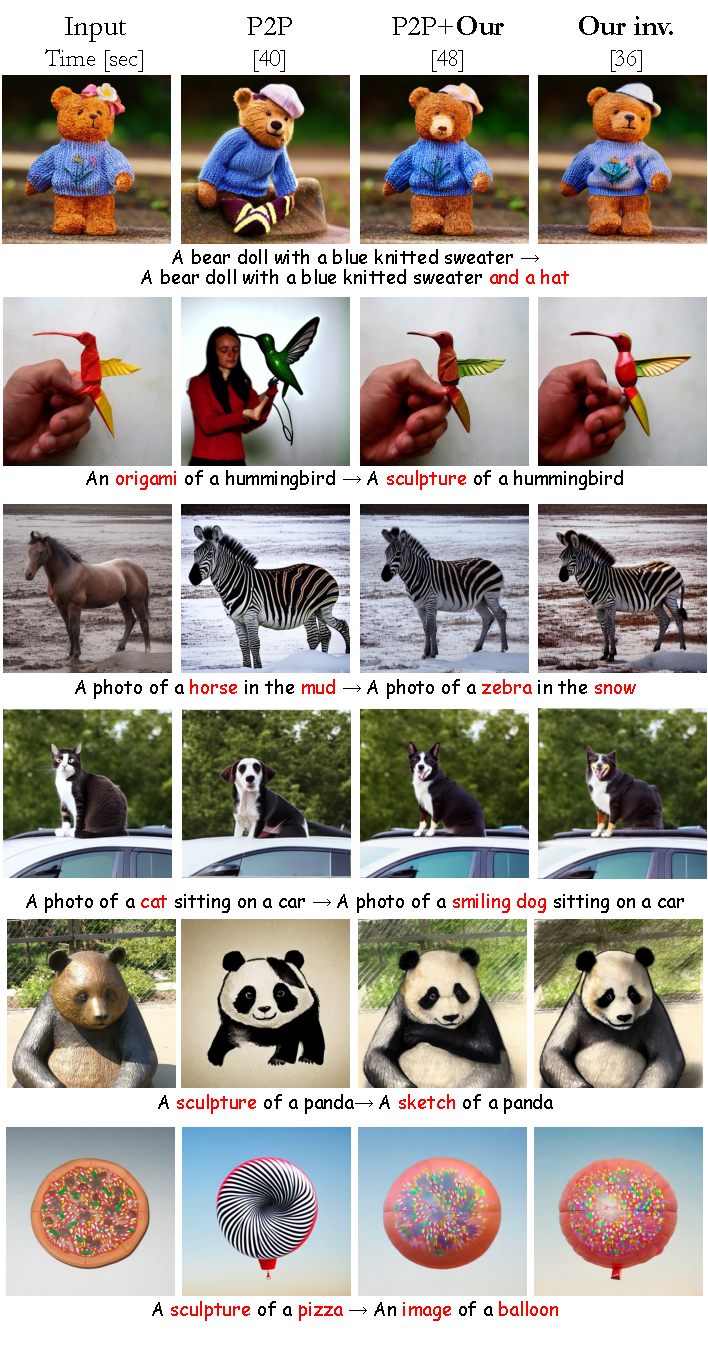
\includegraphics[width=0.65\textwidth]{ICCV23_submission/figures/p2p_1.pdf}
\caption{\textbf{Comparison to P2P, with and without our inversion}. }
\label{fig:p2p_1}
\end{figure}

\clearpage


\begin{figure}
\centering
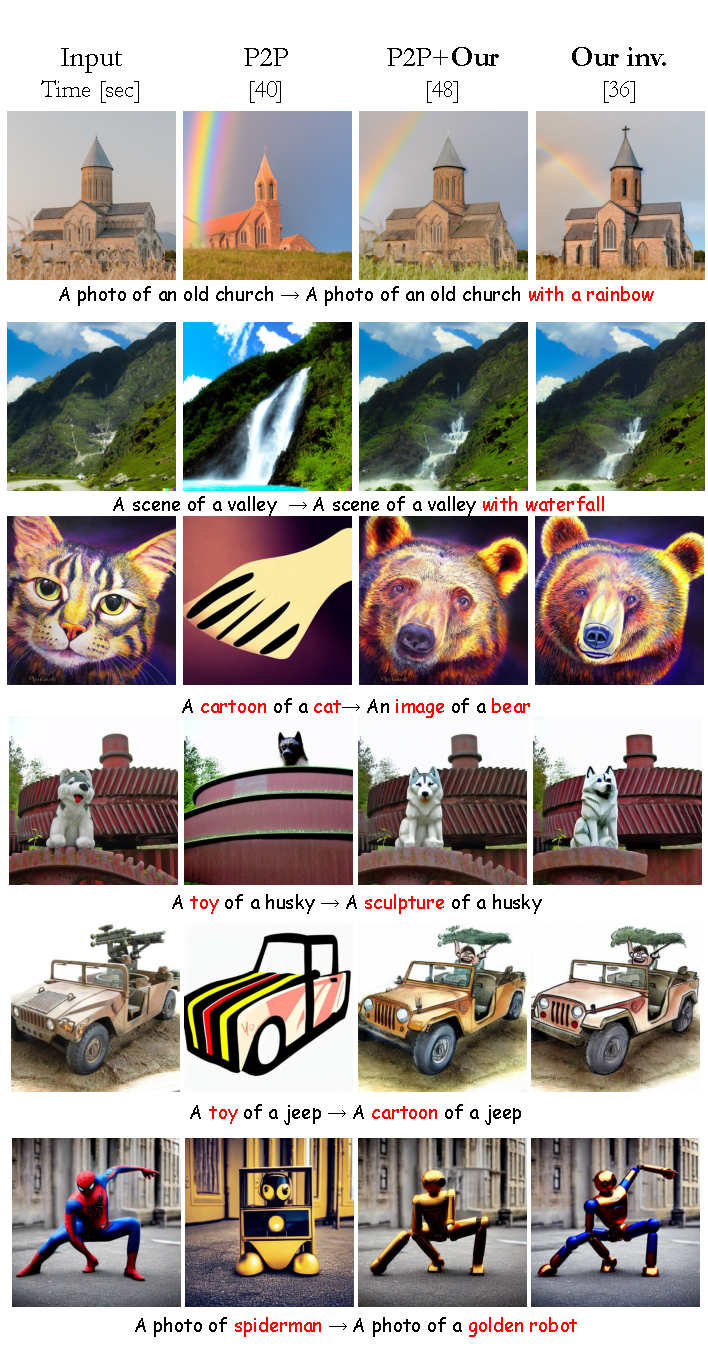
\includegraphics[width=0.65\textwidth]{ICCV23_submission/figures/p2p_2.pdf}
\caption{\textbf{Additional comparisons to P2P, with and without our inversion}. }
\label{fig:p2p_2}
\end{figure}

\clearpage

\clearpage
\section{Additional details on experiments and further numerical evaluation} 
\label{app:AdditionalDetails}
For all our text-based editing experiments, we used Stable Diffusion as our pre-trained text-to-image model. We specifically used the StableDiffusion-v-1-4 checkpoint. We ran all experiments on an RTX A6000 GPU. We now provide additional details about the evaluations reported in the main text. All datasets and prompts will be published.

In addition to measuring CLIP-based scores, LPIPS scores, and running time, we also measure the diversity among generated outputs (higher is better). Specifically, for each image and source text $p_{\text{src}}$, we generate 8 outputs with target text $p_{\text{tar}}$ and calculate the average LPIPS distance over all $\begin{psmallmatrix}8\\2\end{psmallmatrix}$ pairs.

\subsection{Experiments on the modified ImageNet-R-TI2I}\label{app:ImageNet-Dataset}
Our modified ImageNet-R-TI2I dataset contains 44 images: 30 taken from PnP~\cite{Narek22}, and 14 from the Internet and from the code bases of other existing text-based editing methods. We verified that there is a reasonable source and target prompt for each image we added. For P2P~\cite{Hertz22} (with and without our inversion), we used the first 30 images with the ``replace'' option, since they were created with rendering and class changes. That is, the text prompts were of the form ``a $\ll$rendering$\gg$ of a $\ll$class$\gg$'' (\eg ``a sketch of a cat'' to ``a sculpture of a cat''). The last 14 images include prompts with additional tokens and different prompt lengths (\eg changing ``A photo of an old church'' to ``A photo of an old church with a rainbow''). Therefore for those images we used the ``refine'' option in P2P. We configured all methods to use 100 forward and backward steps, except for PnP whose supplied code does not work when changing this parameter. 

Table~\ref{tab:table_parameter} summarizes the hyper-parameters we used for all methods. These apply to both the numerical evaluations and to the visual results shown in the figures. For our inversion, for P2P with our inversion, and for CycleDiffusion we arrived at those parameters by experimenting with various sets of parameters and choosing the configuration that led to the best CLIP loss under the constraint that the LPIPS distance does not exceed $0.3$. For DDIM inversion and for P2P (who did not illustrate their method on real images), such a requirement could not be satisfied. Therefore for those methods we chose the configuration that led to the best CLIP loss under the constraint that the LPIPS distance does not exceed $0.62$. We show results over DDIM inversion with 100 and 50 number of diffusion steps. For DDIM inversion mid-way we use the inversion until a specific timestep. For PnP, null-text inversion, and EDICT we used the default parameters supplied by the authors.


% In this graph, we show three different parameter configurations for our inversion, for P2P with our inversion, and for CycleDiffusion. As can be seen, our method (by itself or with P2P) achieves the best LPIPS distance for any given level of CLIP similarity.

\begin{table}[H]
\centering
\small
\begin{tabular}{| c | c c | c c c|} 
 \hline
 \multirow{2}*{Method} & $\#$inv. & $\#$edit &  \multirow{2}*{strength} &  \multirow{2}*{$T_{\text{skip}}$}&  \multirow{2}*{$\tau_{\text{x}} \slash \tau_{\text{a}}$} \\
&steps & steps&& &

 \\[0.5ex]
 \hline\hline
 %\hline
  DDIM inv. $(T=100)$ &100 & 100 & 9& 0 & -- \\
  DDIM inv. $(T=50)$ &50 & 50 & 9& 0 & -- \\
P2P & 100& 100 & 9 & 0 & 80\slash40 \\ 
%\hline
P2P + Our inv. &100 &100  & 9 & 12 & 60\slash20\\ 
 PnP & 1000 & 50 & 10 & 0 & 40\slash25 \\ 
 EDICT & 50 & 50 & 3 & 10 & --- \\ 
null-text inversion & 50 & 50 & 7.5 & 0 & 80\slash40 \\ 
%\hline
 CycleDiffusion $(\eta=0.1)$ & 100 & 100 & 3 & 30 & -- \\  %\hline
 CycleDiffusion $(\eta=1.0)$ & 100 & 100 & 3 & 30 & -- \\  %\hline
%\hline
Our inv. & 100 & 100 & 15 & 36 & --\\

\hline
\end{tabular}
\caption{\textbf{Hyper-parameters used in experiments on the modified ImageNet-R-TI2I dataset}. The parameter `strength' refers to the classifier-free scale of the generation process. As for the strength used in the inversion stage, we set it to $3.5$ for all methods except for PnP and CycleDiffusion which uses $1$. The timestep at which we start the generation is $T-T_{\text{skip}}$ and, in case of injecting attentions, we also report the timesteps determine until which step (starting from zero) the cross- and self-attentions are injected, $\tau_{\text{x}}$ and $\tau_{\text{a}}$ respectively.}
\label{tab:table_parameter}
\end{table}

% \begin{table}[H]
% \centering
% \small
% \begin{tabular}{| c | c c c|} 
%  \hline
%  Method & strength & $T_{\text{skip}}$ &  $\tau_{\text{x}} \slas \tau_{\text{a}}$ \\
%  % \\[0.5ex]
%  \hline\hline
%  %\hline
%   DDIM inv. & 9& 0 & -- \\
% P2P & 9 & 0 & 80\slash40 \\ 
% %\hline
% P2P + Our inv.   & 9 & 12 & 60\slash20\\ 
%  PnP  & 10 & 0 & 40\slash25 \\ 
%  EDICT  & 3 & 10 & --- \\ 
% null-text inversion & 7.5 & 0 & 80\slash40 \\ 
% %\hline
%  CycleDiffusion $(\eta=0.1)$  & 3 & 30 & -- \\  %\hline
%  CycleDiffusion $(\eta=1.0)$ & 3 & 30 & -- \\  %\hline
% %\hline
% Our inv. & 15 & 36 & --\\
% \hline
% \end{tabular}
% \caption{\textbf{Hyper-parameters used in experiments on the modified ImageNet-R-TI2I dataset}. The parameter `strength' refers to the classifier-free scale of the generation process. As for the strength used in the inversion stage, we set it to $3.5$ for all methods except for PnP and CycleDiffusion which uses $1$. The timestep at which we start the generation is $T-T_{\text{skip}}$ and, in case of injecting attentions, we also report the timesteps determine until which step (starting from zero) the cross- and self-attentions are injected, $\tau_{\text{x}}$ and $\tau_{\text{a}}$ respectively.}
% \label{tab:table_parameter}
% \end{table}

Table~\ref{tab:comparison_table} and Figure~\ref{fig:clip_lpips_all} summarizes the comparisons of all methods reported in the paper with the hyper-parameters from Tab~\ref{tab:table_parameter}. The results show that our inversion achieves a good balance between LPIPS and CLIP, while requiring short edit times. Integrating our inversion into P2P improves their performance in both metrics. Our method, CycleDiffusion, and null-text inversion support diversity among generated outputs.

\begin{table}[H]
\centering
\footnotesize
\begin{tabular}{| c | c c c c|} 
 \hline
 Method & CLIP sim.$\uparrow$ & LPIPS$\downarrow$ & Diversity$\uparrow$ & Time$\downarrow$ \\[0.5ex]
 \hline\hline
 DDIM inv. $(T=100)$  & 0.31 & 0.62 & 0.00 & 39\\
 DDIM inv. $(T=50)$  & 0.31 & 0.62 & 0.00 & 39\\
 P2P & 0.30 & 0.61 & 0.00 & 40\\
 \bf{P2P+Our}  & 0.31 & \bf{0.25} & 0.11 & 48\\  %[1ex] 
 PnP & 0.31 & 0.36 & 0.00 & 206\\ 
 EDICT & 0.29 & 0.27 & 0.00 & 520\\ 
 null-text inversion & 0.29 & 0.35 & 0.08 & 160\\ 
 CycleDiffusion, \!$\eta\!=\!0.1$ & 0.30 & 0.27 & 0.21 &  \bf{36}\\ 
 CycleDiffusion, \!$\eta\!=\!1.0$ & 0.30 & 0.26 & \bf{0.306} &  \bf{36}\\ 
 %\hline
%\hline
\bf{Our inv.}  & \bf{0.32} &0.29 & 0.18 & \bf{36}\\
%\hline
%\hline
\hline
% \bf{Our inv.} & 9 & 36 & 0.32 & 0.24 & ?\\ 
% \hline
\end{tabular}
\caption{Evaluation on modified ImageNet-R-TI2I dataset.}
\label{tab:comparison_table}
\end{table}


% In this experiment, we follow the default scale parameter of classifier-free and set it to be 3.5 for the forward (the inversion part) in all methods \inbar{ask vova if also pnp}. 

\begin{figure}[h]
\centering
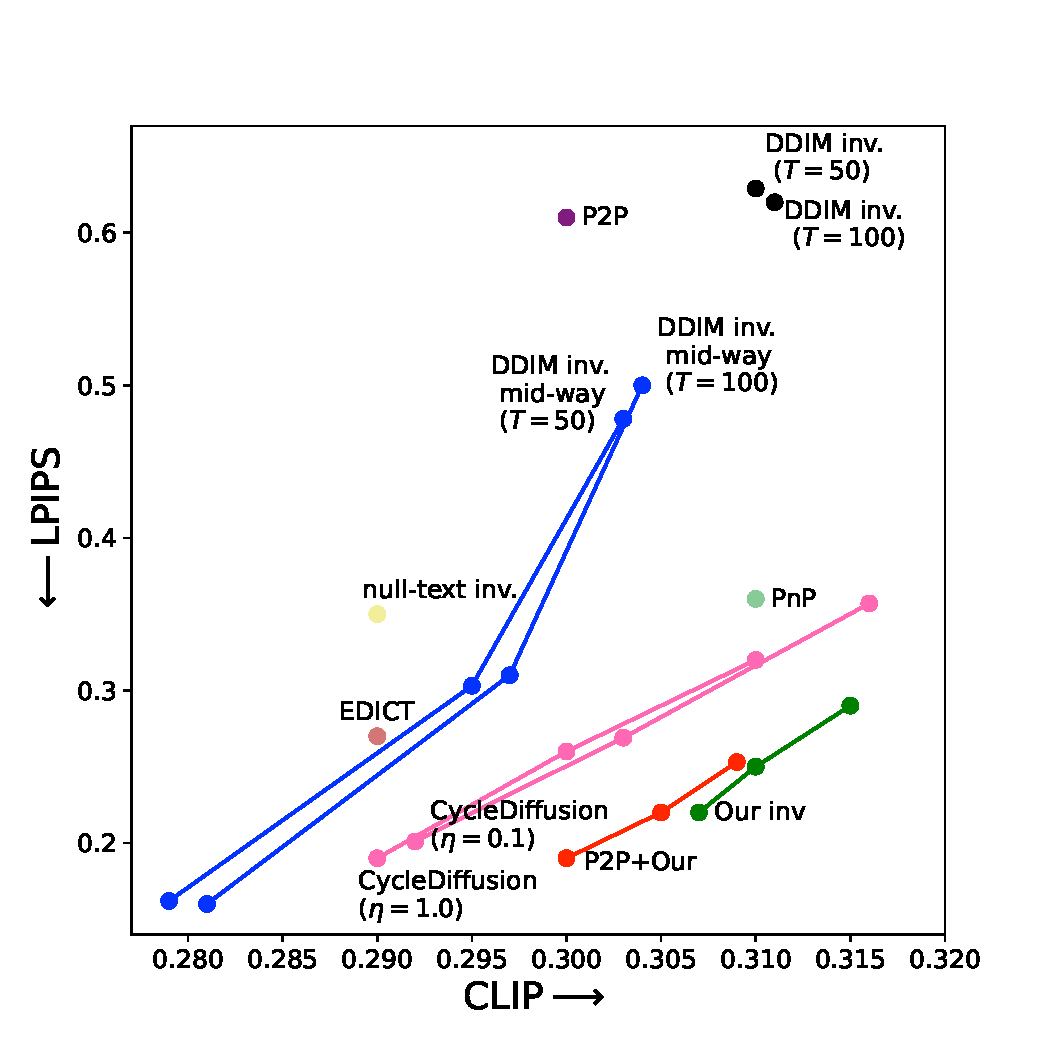
\includegraphics[width=0.7\columnwidth]{ICCV23_submission/figures/clip_lpips_all.pdf}
\caption{\textbf{Fidelity to source image vs.~compliance with target text.} We show a comparison of all methods.}% The standard-deviation of the CLIP measurements varied between $0.007$ and $0.048$ for all methods, and standard deviations of the LPIPS loss varied between $0.097$ and $0.135$.}
\label{fig:clip_lpips_all}
\end{figure}

\clearpage

\subsection{Experiments on the modified zero-shot I2IT dataset}\label{app:zero-shot-dataset}
The second dataset we used is the modified Zero-Shot I2IT dataset, which contains 4 categories (cat, dog, horse, zebra). Ten images from each category were taken from Parmar \etal~\cite{Parmar23}, and we added 5 more images from the Internet to each category. Zero-Shot I2I~\cite{Parmar23} does not use source-target pair prompts, but rather pre-defined source-target classes (\eg cat$\leftrightarrow$dog). For their optimized DDIM-inversion part, they use a source prompt automatically generated with BLIP~\cite{Junnan22}. When combining our inversion with their generative method, we use $T_{\text{skip}}=0$ and an empty source prompt. Table~\ref{tab:table_parameter_zero_shot} summarizes the hyper-parameters used in every method.

% \begin{table}[H]
% \centering
% \small
% \begin{tabular}{| c |c c c|} 
%  \hline
%  Method & strength & $T_{\text{skip}}$& $\lambda_{\text{xa}}$ \\
%  % \\[0.5ex]
%  \hline\hline
%  Zero-Shot & 7.5 & 0 & 0.1 \\ 
%  %\hline
% Zero-Shot+Our& 7.5 & 0 & 0.03 \\
% %\hline
% \hline
% % \bf{Our inv.} & 9 & 36 & 0.32 & 0.24 & ?\\ 
% % \hline
% \end{tabular}
% \caption{\textbf{Hyper-parameters used in experiments on the modified Zero-Shot I2IT dataset}. In this method, cross-attention guidance weight is the parameter used to control the consistency in the cross-attention maps, denoted here as $\lambda_{\text{xa}}$. We set the strength (classifier-free scale) in the inversion part to be $1$ and $3.5$ for ``Zero-shot'' and ``Zero-shot+Our'' respectively.}
% \label{tab:table_parameter_zero_shot}
% \end{table}

\begin{table}[H]
\centering
\small
\begin{tabular}{| c | c c | c c c|} 
 \hline
 \multirow{2}*{Method} & $\#$inv. & $\#$edit &  \multirow{2}*{strength} &  \multirow{2}*{$T_{\text{skip}}$}&  \multirow{2}*{$\lambda_{\text{xa}}$} \\
&steps & steps&& &

 \\[0.5ex]
 \hline\hline
 Zero-Shot & 50 & 50 & 7.5 & 0 & 0.1 \\ 
 %\hline
Zero-Shot+Our &50 & 50 & 7.5 & 0 & 0.03 \\
%\hline
\hline
% \bf{Our inv.} & 9 & 36 & 0.32 & 0.24 & ?\\ 
% \hline
\end{tabular}
\caption{\textbf{Hyper-parameters used in experiments on the modified Zero-Shot I2IT dataset}. In this method, cross-attention guidance weight is the parameter used to control the consistency in the cross-attention maps, denoted here as $\lambda_{\text{xa}}$. We set the strength (classifier-free scale) in the inversion part to be $1$ and $3.5$ for ``Zero-shot'' and ``Zero-shot+Our'' respectively.}
\label{tab:table_parameter_zero_shot}
\end{table}

Tab~\ref{tab:comparison_table_zero}
summarizes the comparison to the Zero-shot method. The results show that integrating our inversion improves the 
similarity to the input image while keeping the CLIP accuracy high. We also exhibit non-negligible diversity among the generated outputs


\begin{table}[H]
\centering
\footnotesize
\begin{tabular}{|c | c c c c|} 
 \hline
 Method & CLIP Acc.$\uparrow$ & LPIPS$\downarrow$ & Diversity$\uparrow$ & Time\\
\hline\hline
Zero-Shot  & 0.88 & 0.35 & 0.07 &\bf{45}\\ 
%\hline
\bf{Zero-Shot+Our} & \bf{0.88} & \bf{0.27} & \bf{0.16} & 46\\  %[1ex] 
\hline
% \bf{Our inv.} & 9 & 36 & 0.32 & 0.24 & ?\\ 
% \hline
\end{tabular}
\caption{Evaluation on the modified Zero-Shot I2IT dataset.}
\label{tab:comparison_table_zero}
\end{table}
%\inbar{should we mention the gpu we use?}
\clearpage
\section{Additional results}

%\paragraph{Our method's variability}
Due to the stochastic nature of our method, we can generate diverse outputs, a feature that is not naturally available with methods relying on the DDIM inversion. Figures~\ref{fig:variability1} and~\ref{fig:variability2} show several diverse text-based editing results.  Figures~\ref{fig:comparisons_SM_1} and \ref{fig:comparisons_SM_2} provide further qualitative comparisons between all methods tested on the ImageNet-R-TI2I dataset. 



\begin{figure*}[h]
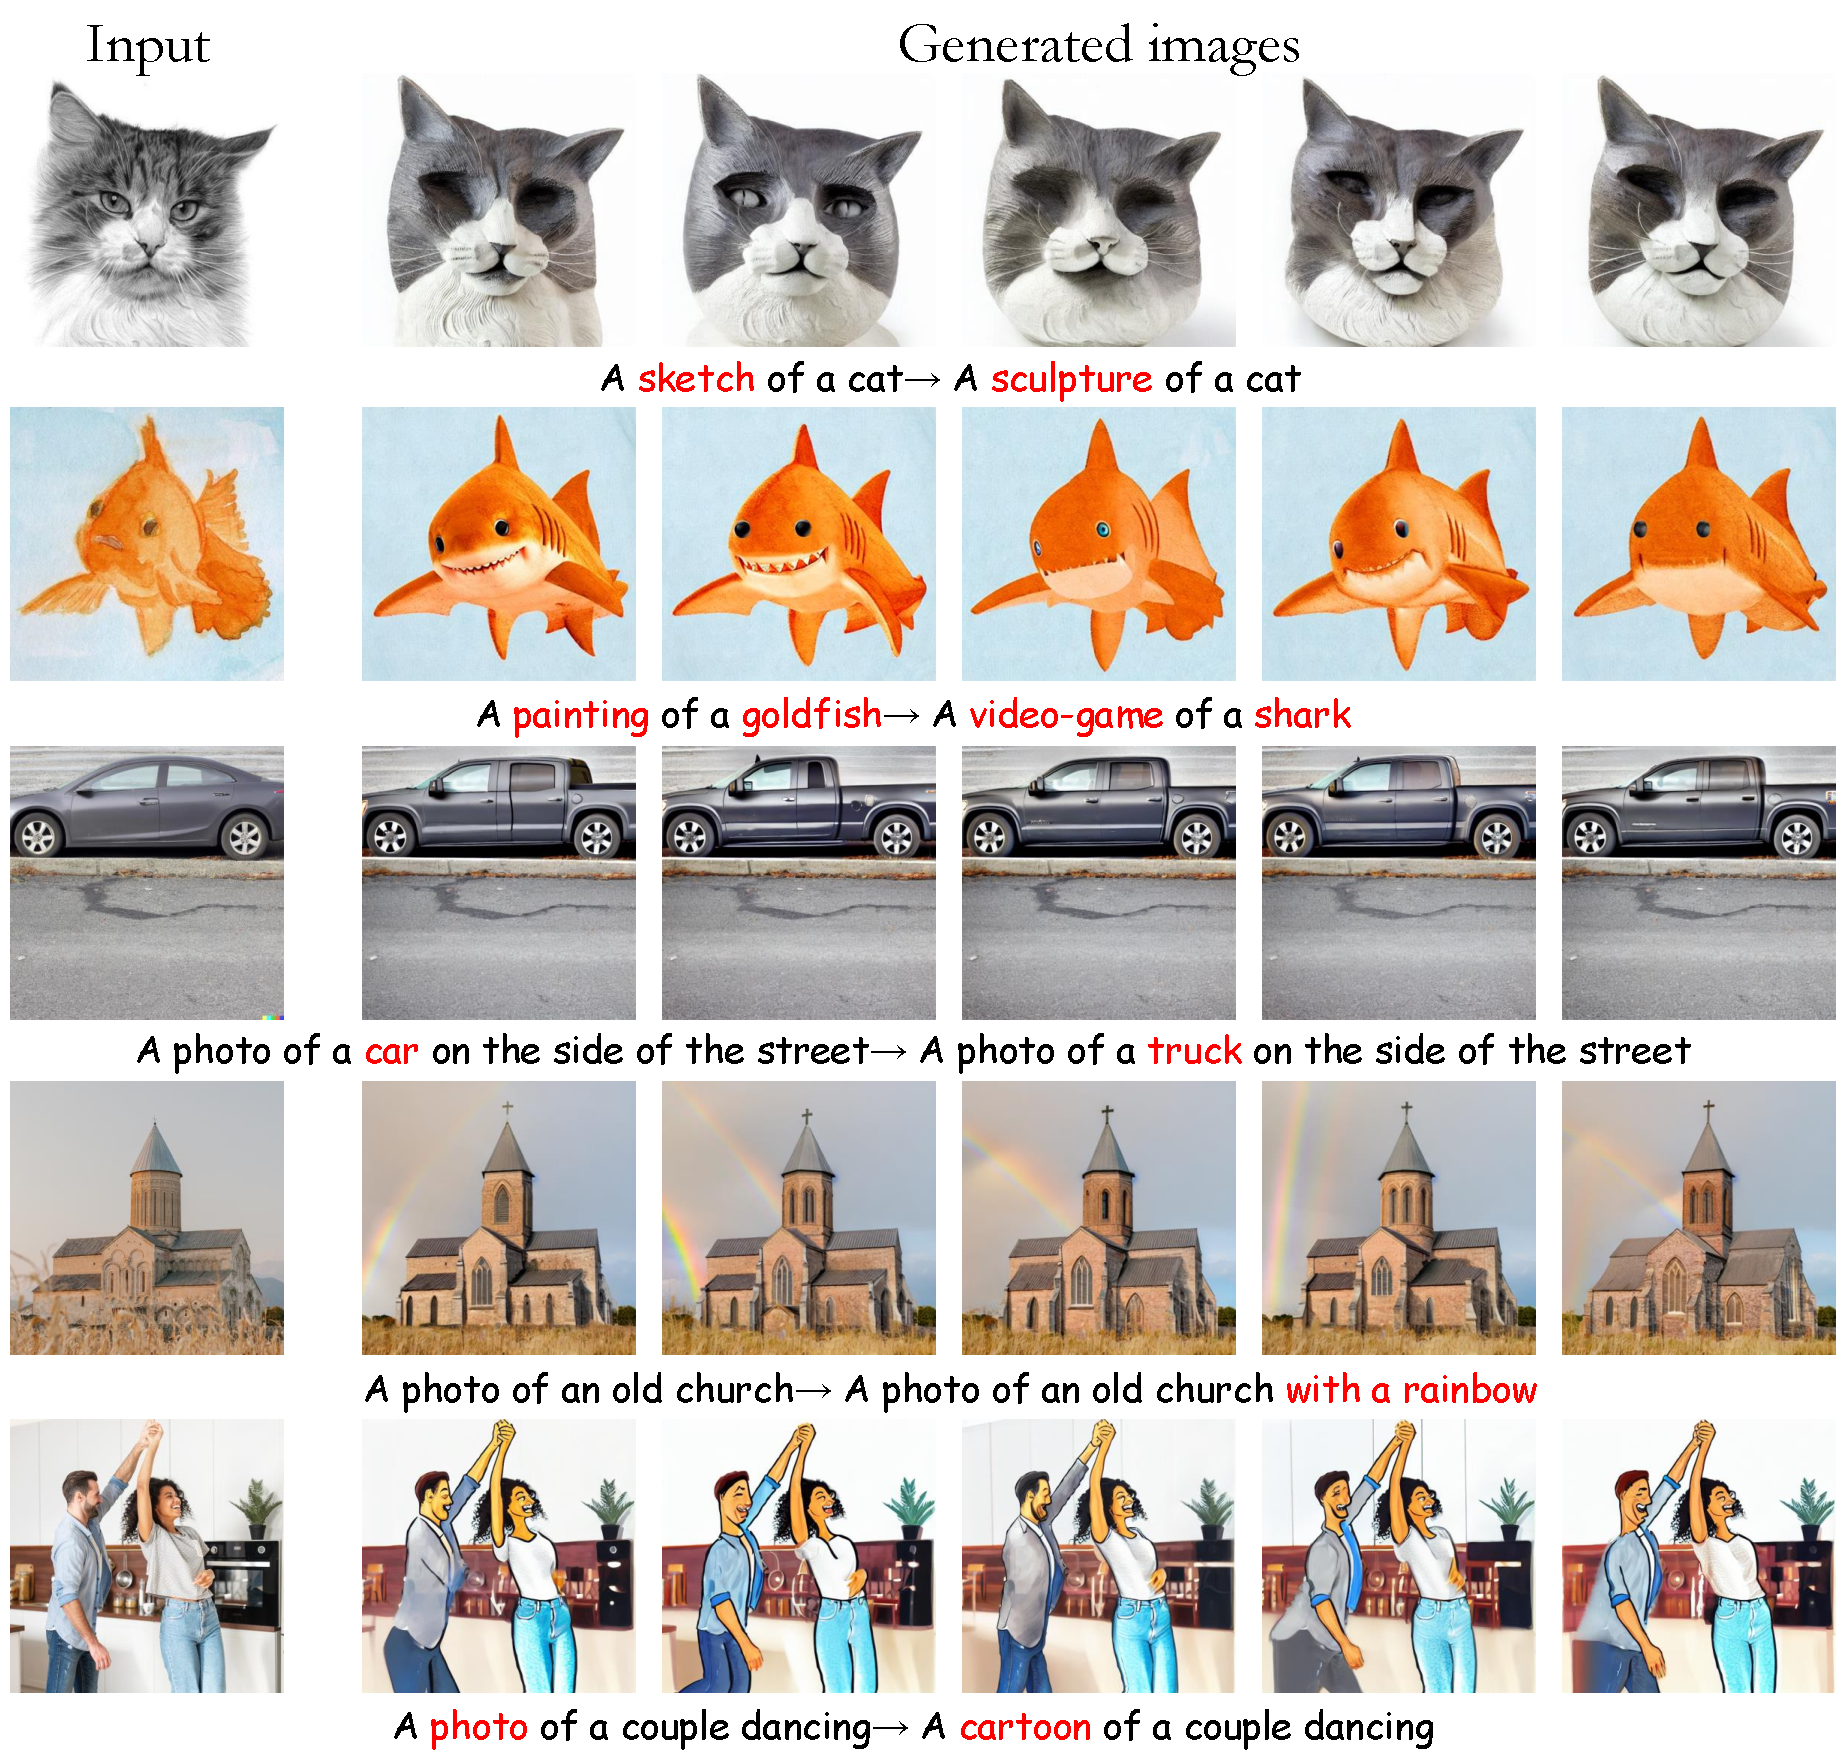
\includegraphics[width=\textwidth]{ICCV23_submission/figures/DDPM_inversion_variability_1.pdf}
\caption{\textbf{Diverse text-based editing with our method}. We apply our inversion five times with the same source and target prompts (shown beneath each example). Note how the variability between the results is not negligible, while all of them conform to the structure of the input image and comply with the target text prompt. Notice \eg the variability in the sculpture cat's eyes and mouth, and how the rainbow appears in different locations and angles.}
\label{fig:variability1}
\end{figure*}

\begin{figure*}
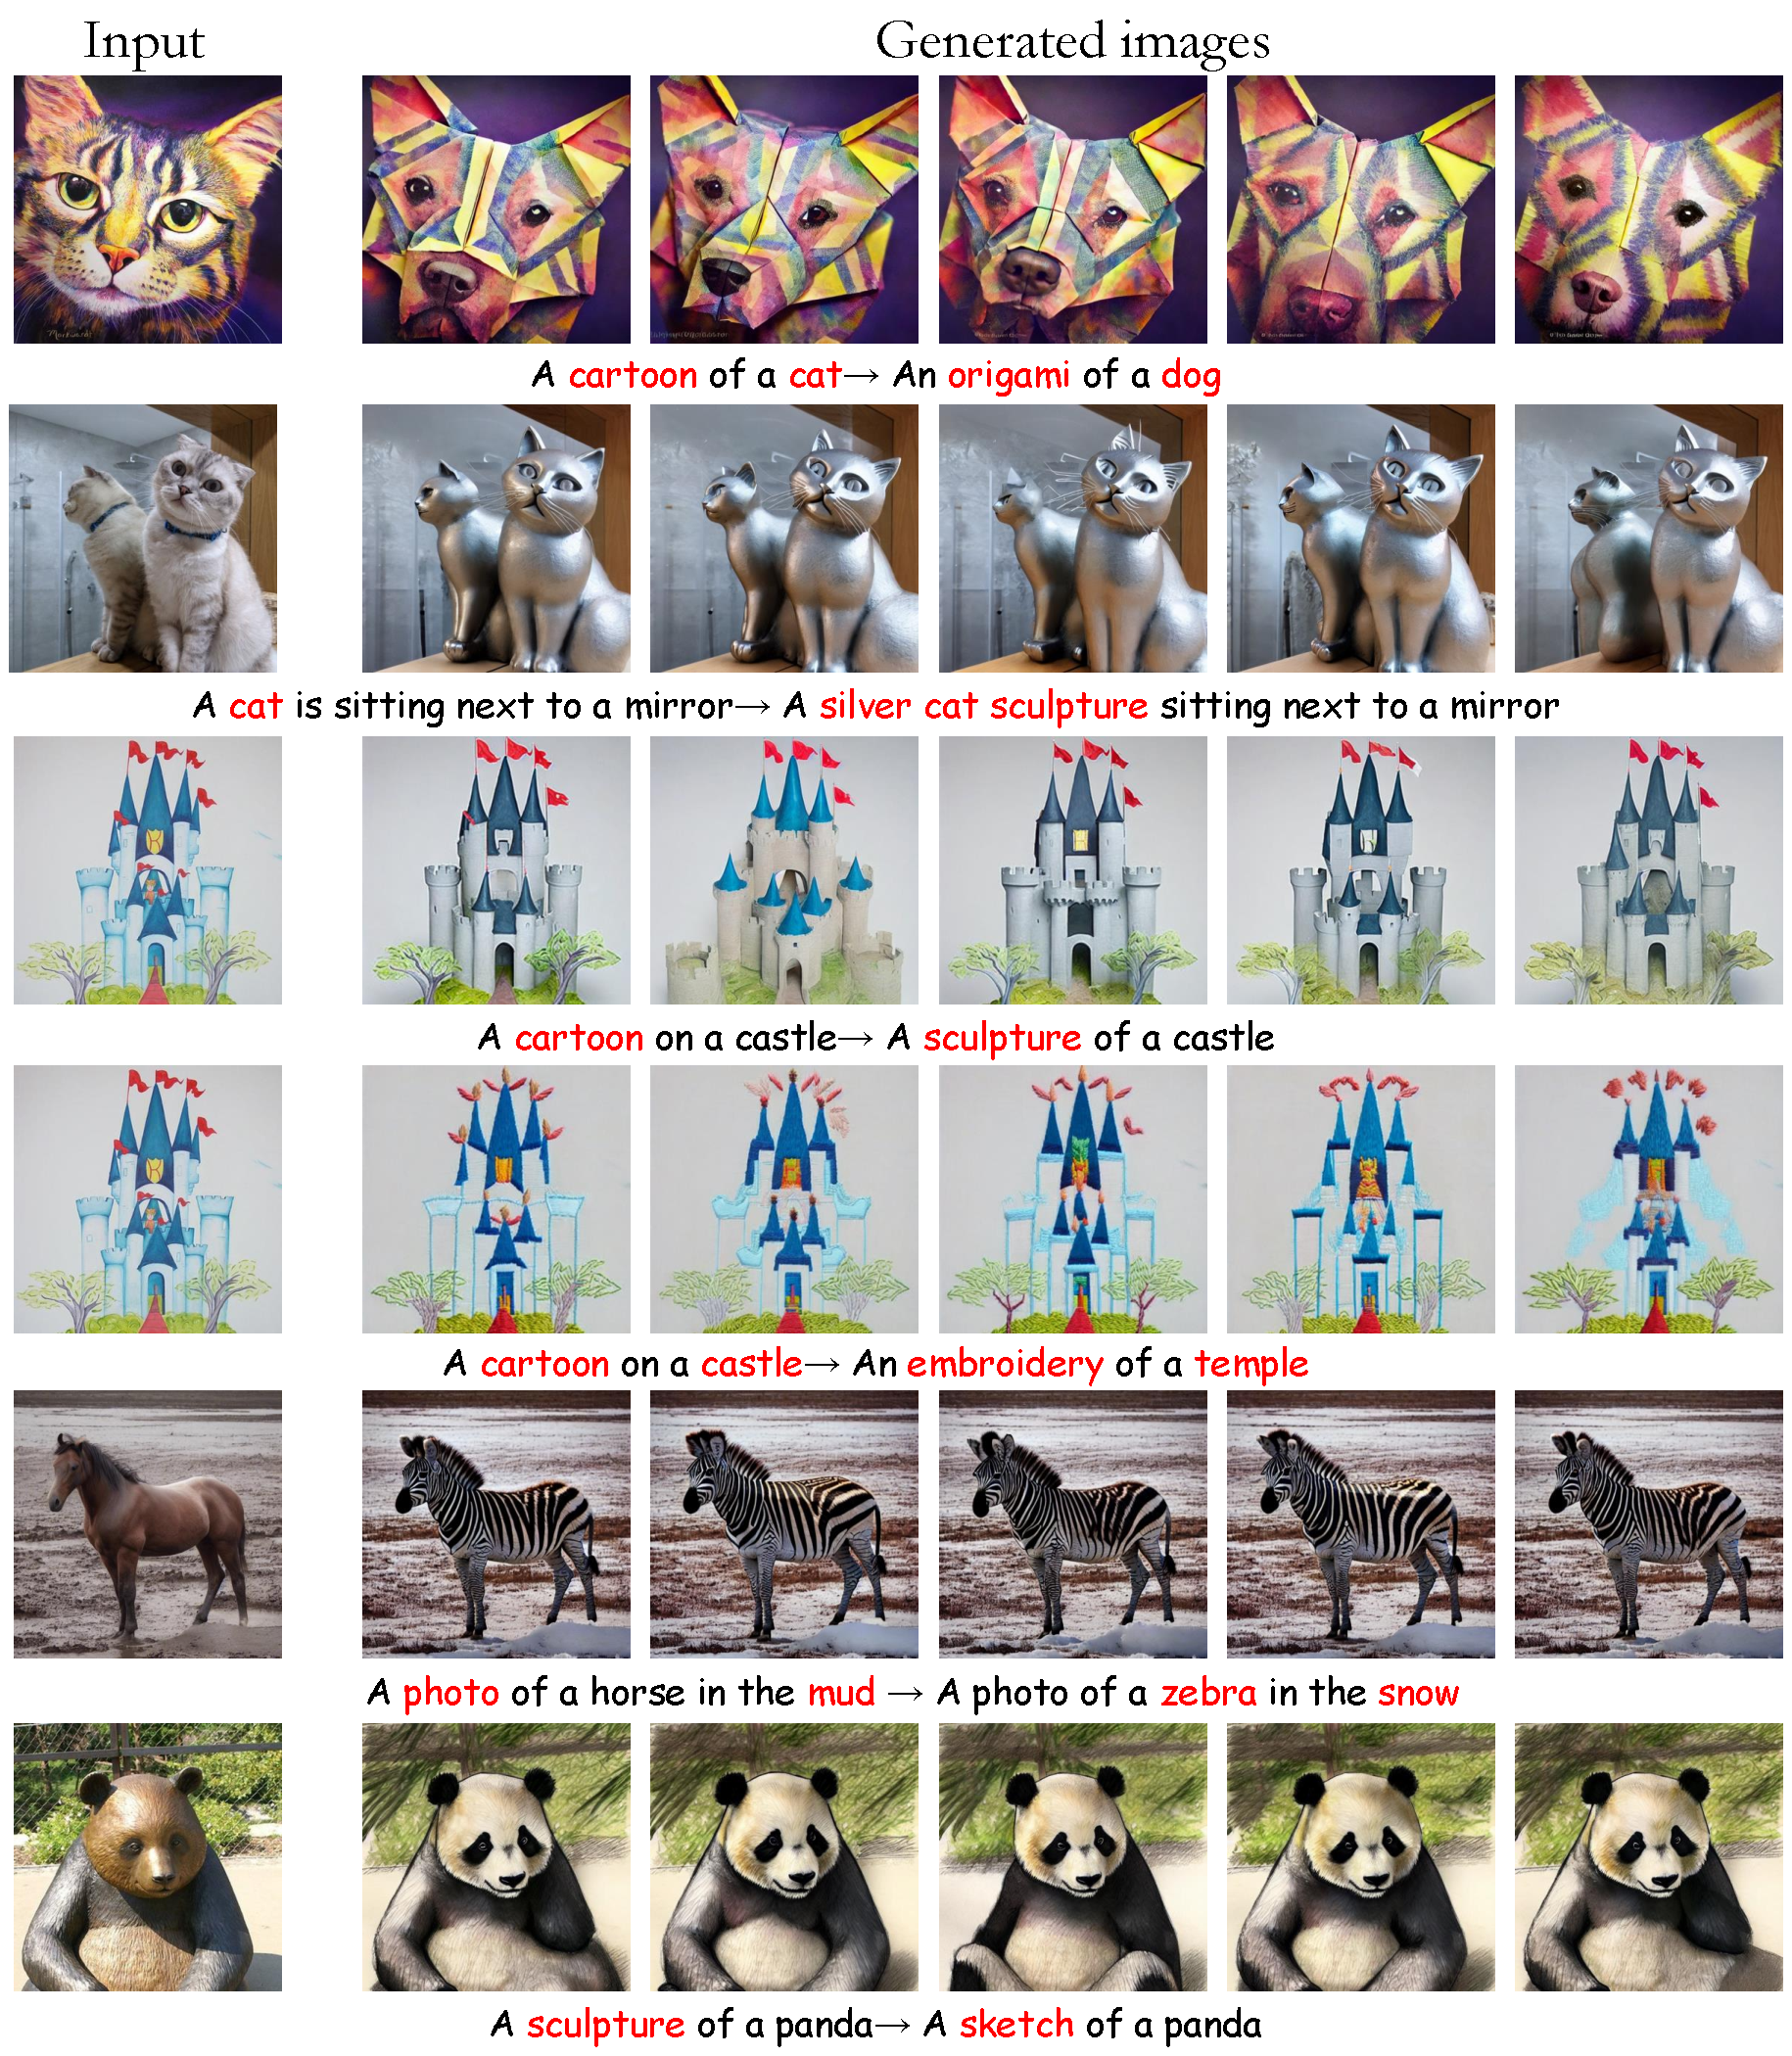
\includegraphics[width=\textwidth]{ICCV23_submission/figures/DDPM_inversion_variability_2.pdf}
\caption{\textbf{Additional results for diverse text-based editing with our method}. Notice that 
each edited result is slightly different. For example, the eyes and nose of the origami dog change between samples, and so do the zebra's stripes.}
\label{fig:variability2}
\end{figure*}

%\paragraph{Comparisons}
%Tab~\ref{tab:comparison_table} shows the average of CLIP and LPIPS scores of all methods on the first dataset. 



% \begin{table}[H]
% \centering
% \small
% \begin{tabular}{| c  | c c |} 
%  \hline
%  Method  & $STD_{\text{CLIP}}$& $STD_{\text{LPIPS}}$ \\[0.5ex]
%  \hline\hline
%  PnP & \textbf{0.007} & 0.135 \\ 
%  %\hline
%  DDIM inv.  & 0.043 & 0.122\\
% %\hline
% \bf{Our inv.}  &  0.035 &0.104\\
% %\hline
% P2P &  0.048 & 0.123\\
% %\hline
% \bf{P2P + Our inv.}  & 0.035 &  \textbf{0.097}\\  [1ex] 
% \hline
% % \bf{Our inv.} & 9 & 36 & 0.32 & 0.24 & ?\\ 
% % \hline
% \end{tabular}
% \caption{\textbf{Standard-devieation of evaluation}.}
% \label{tab:table_std}
% \end{table}




\begin{figure*}[h]
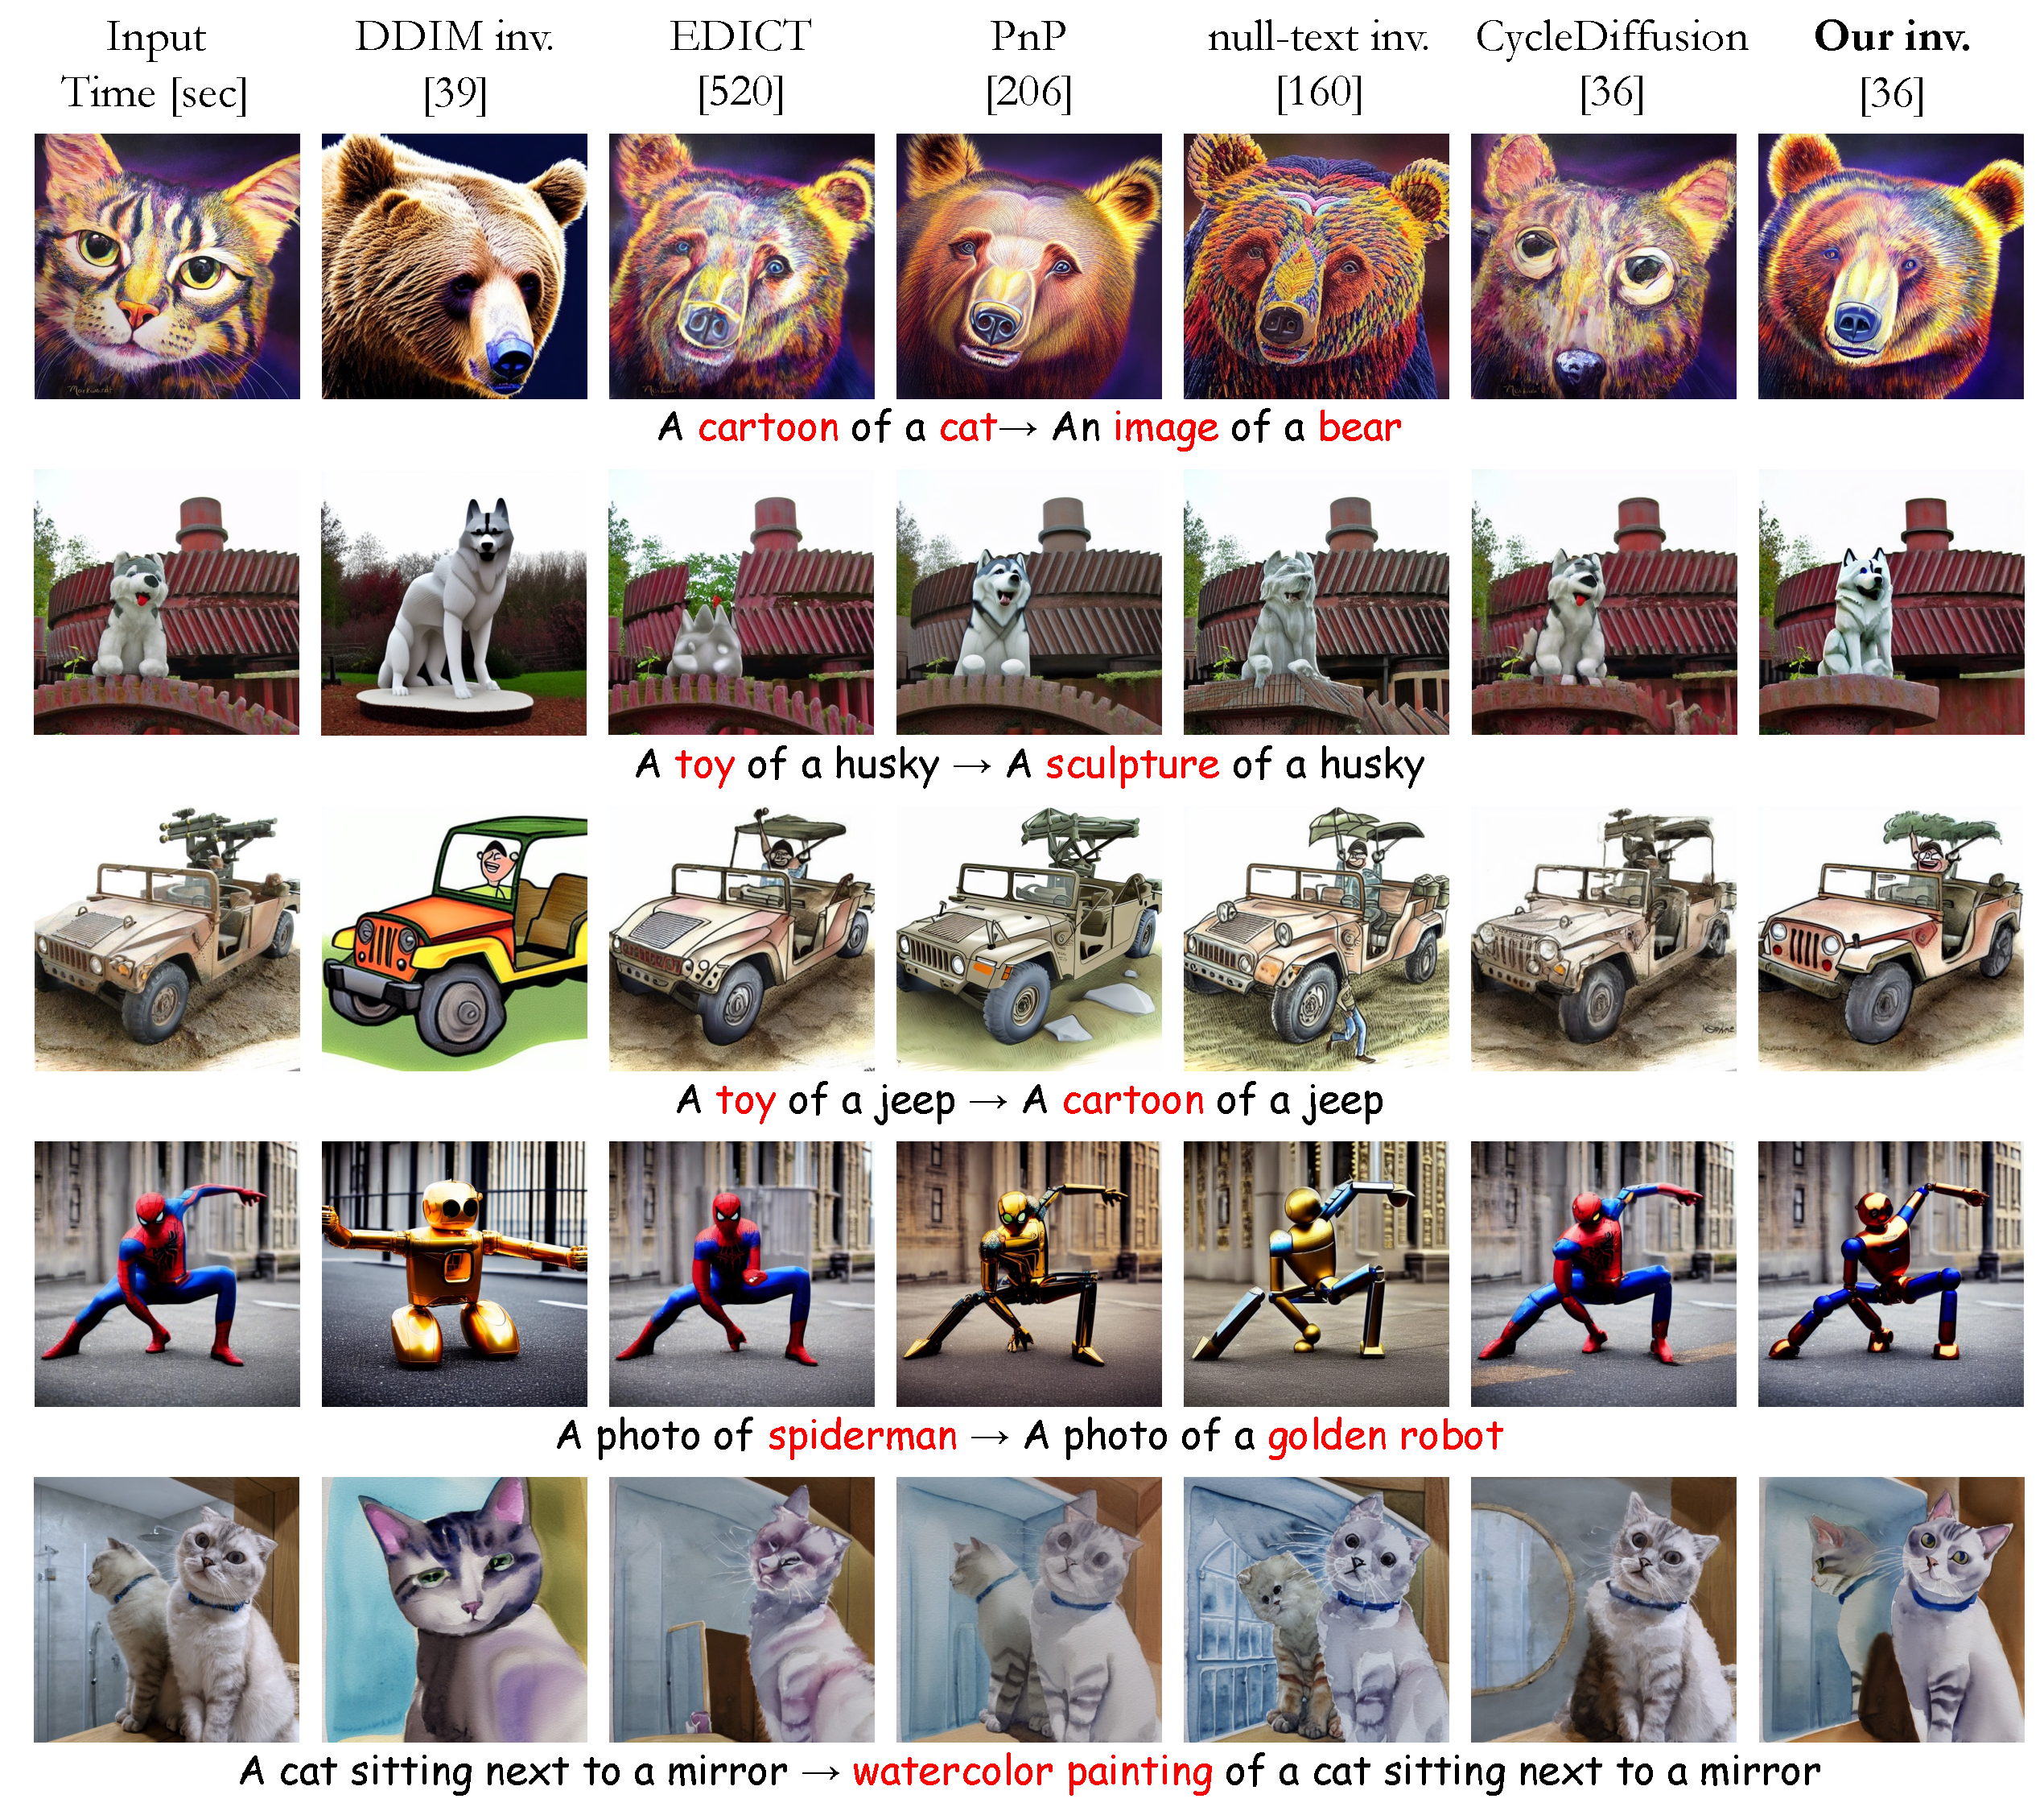
\includegraphics[width=\textwidth]{ICCV23_submission/figures/comparison_SM_1.pdf}
\caption{\textbf{Qualitative comparisons between all methods.}}
\label{fig:comparisons_SM_1}
\end{figure*}

\clearpage

\begin{figure*}[h]
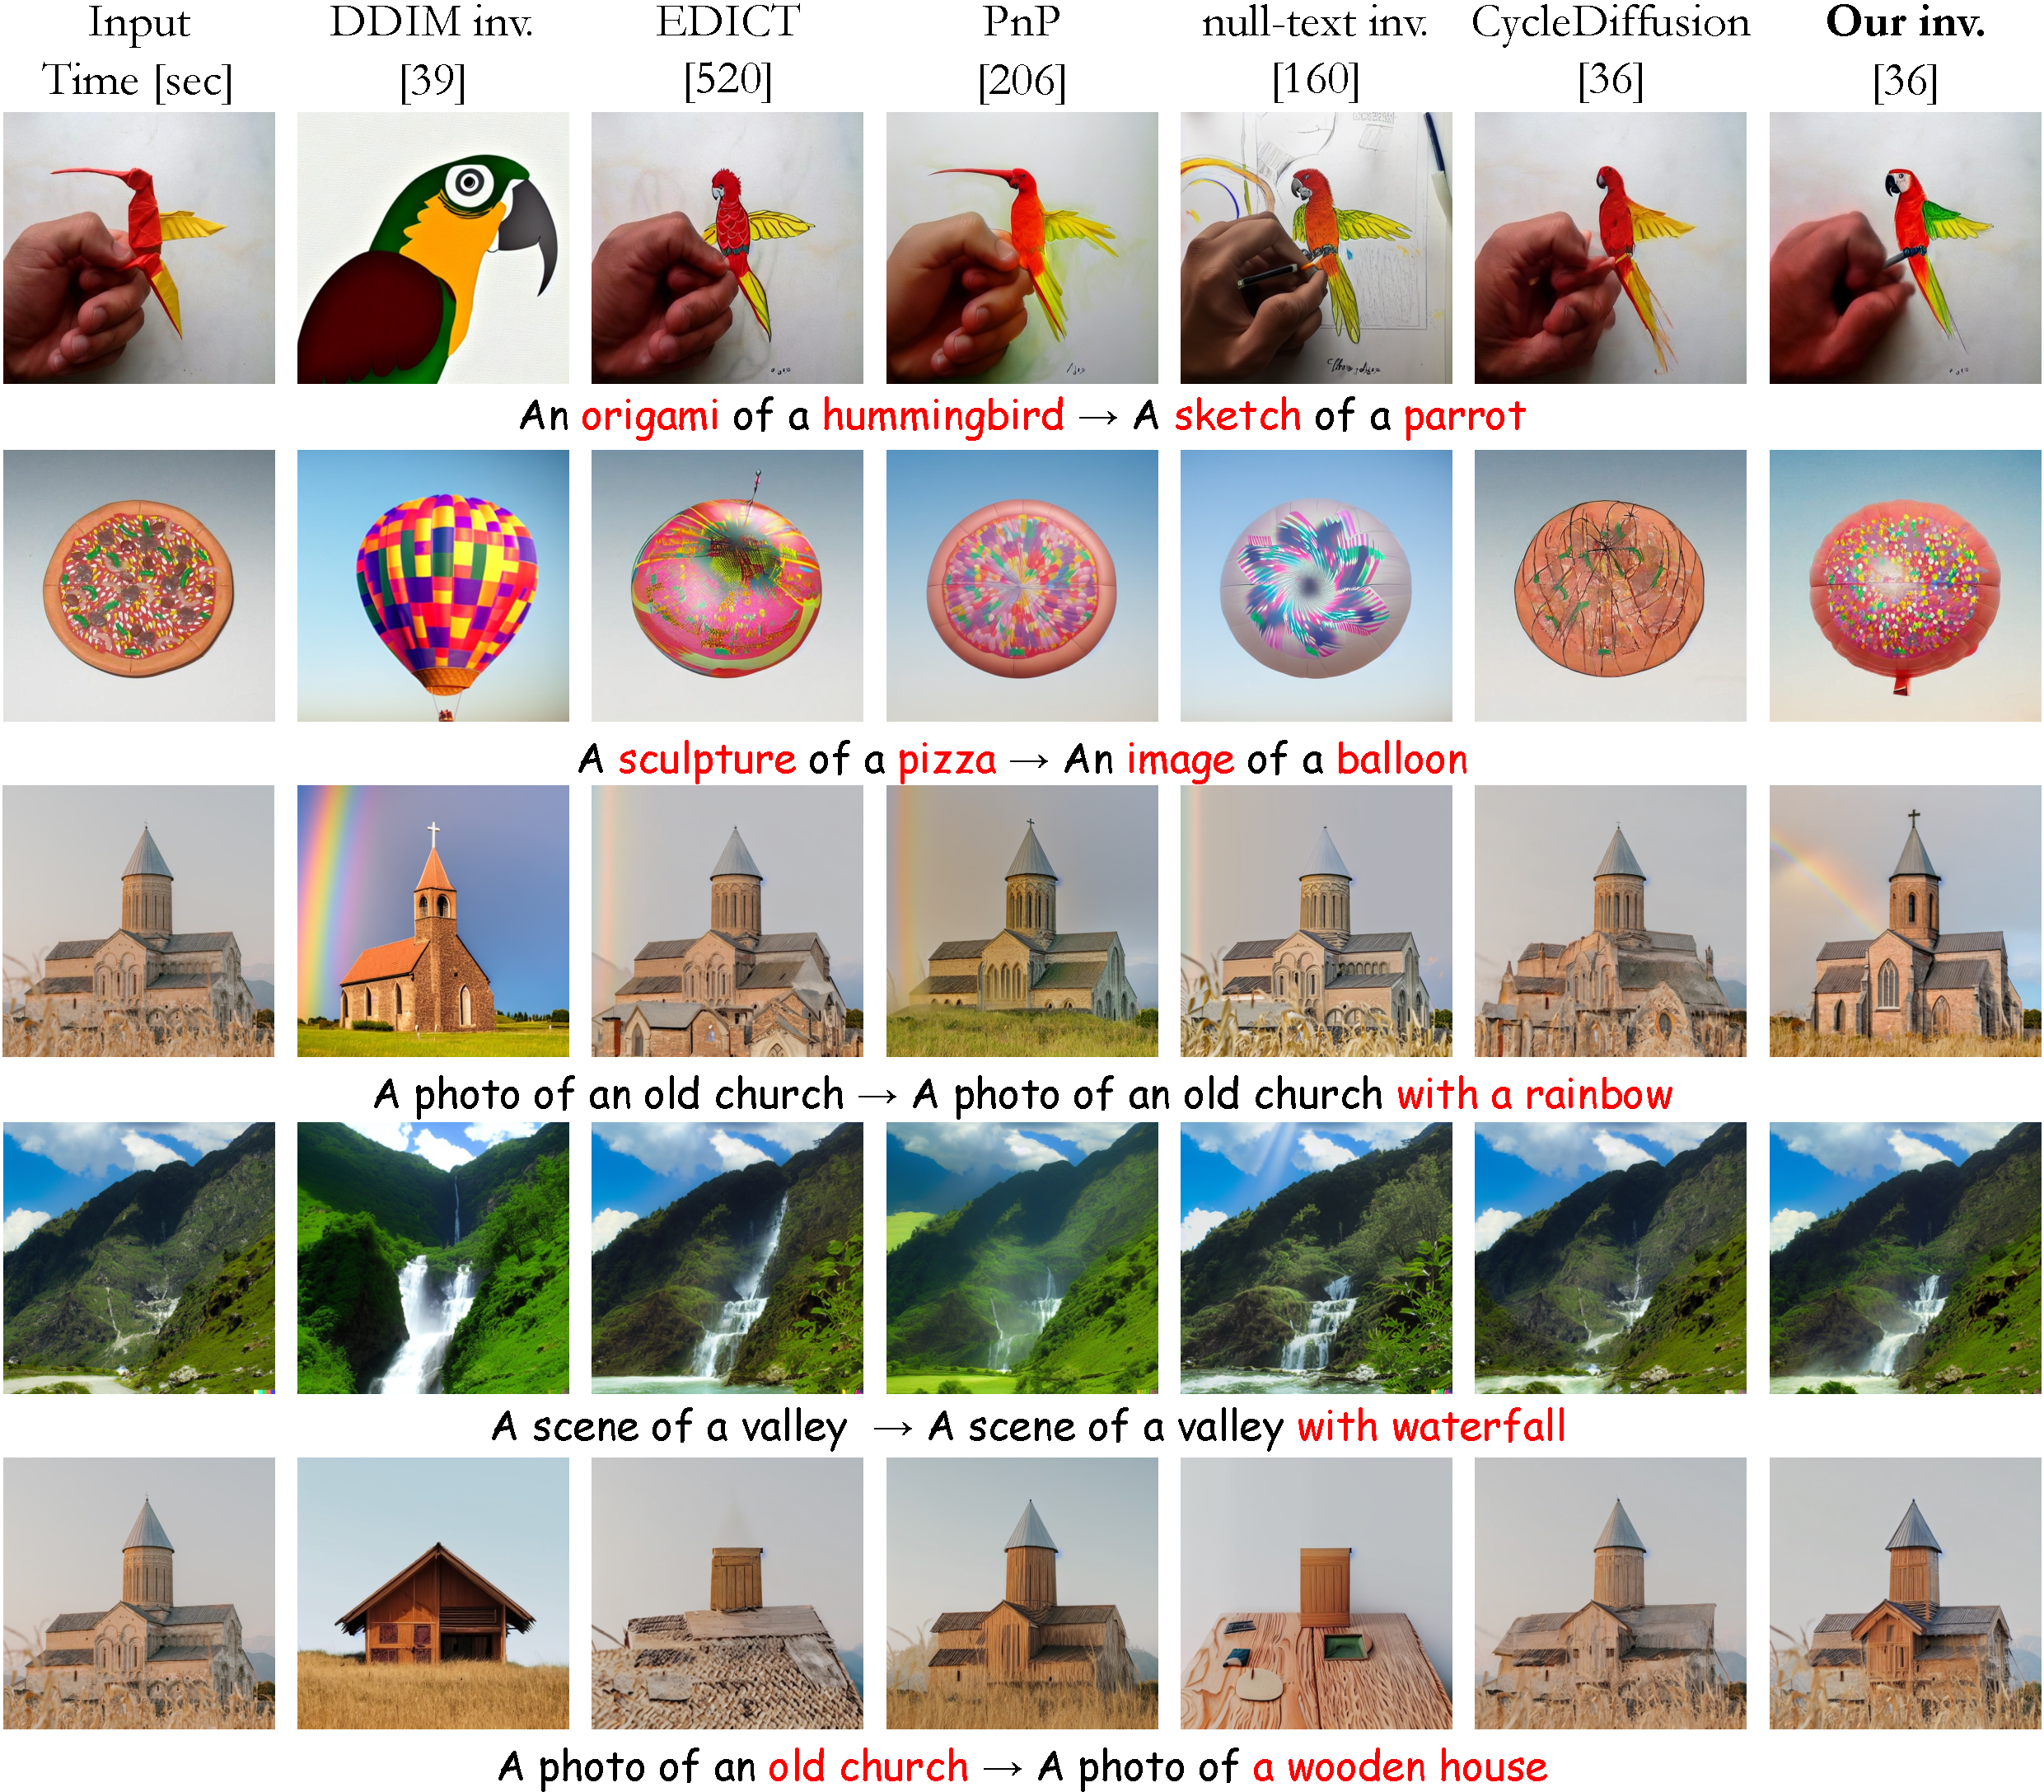
\includegraphics[width=\textwidth]{ICCV23_submission/figures/comparison_SM_2.pdf}
\caption{\textbf{Additional qualitative comparisons between all methods.}}
\label{fig:comparisons_SM_2}
\end{figure*}

\clearpage

% \begin{figure*}[h]
% \centering
% 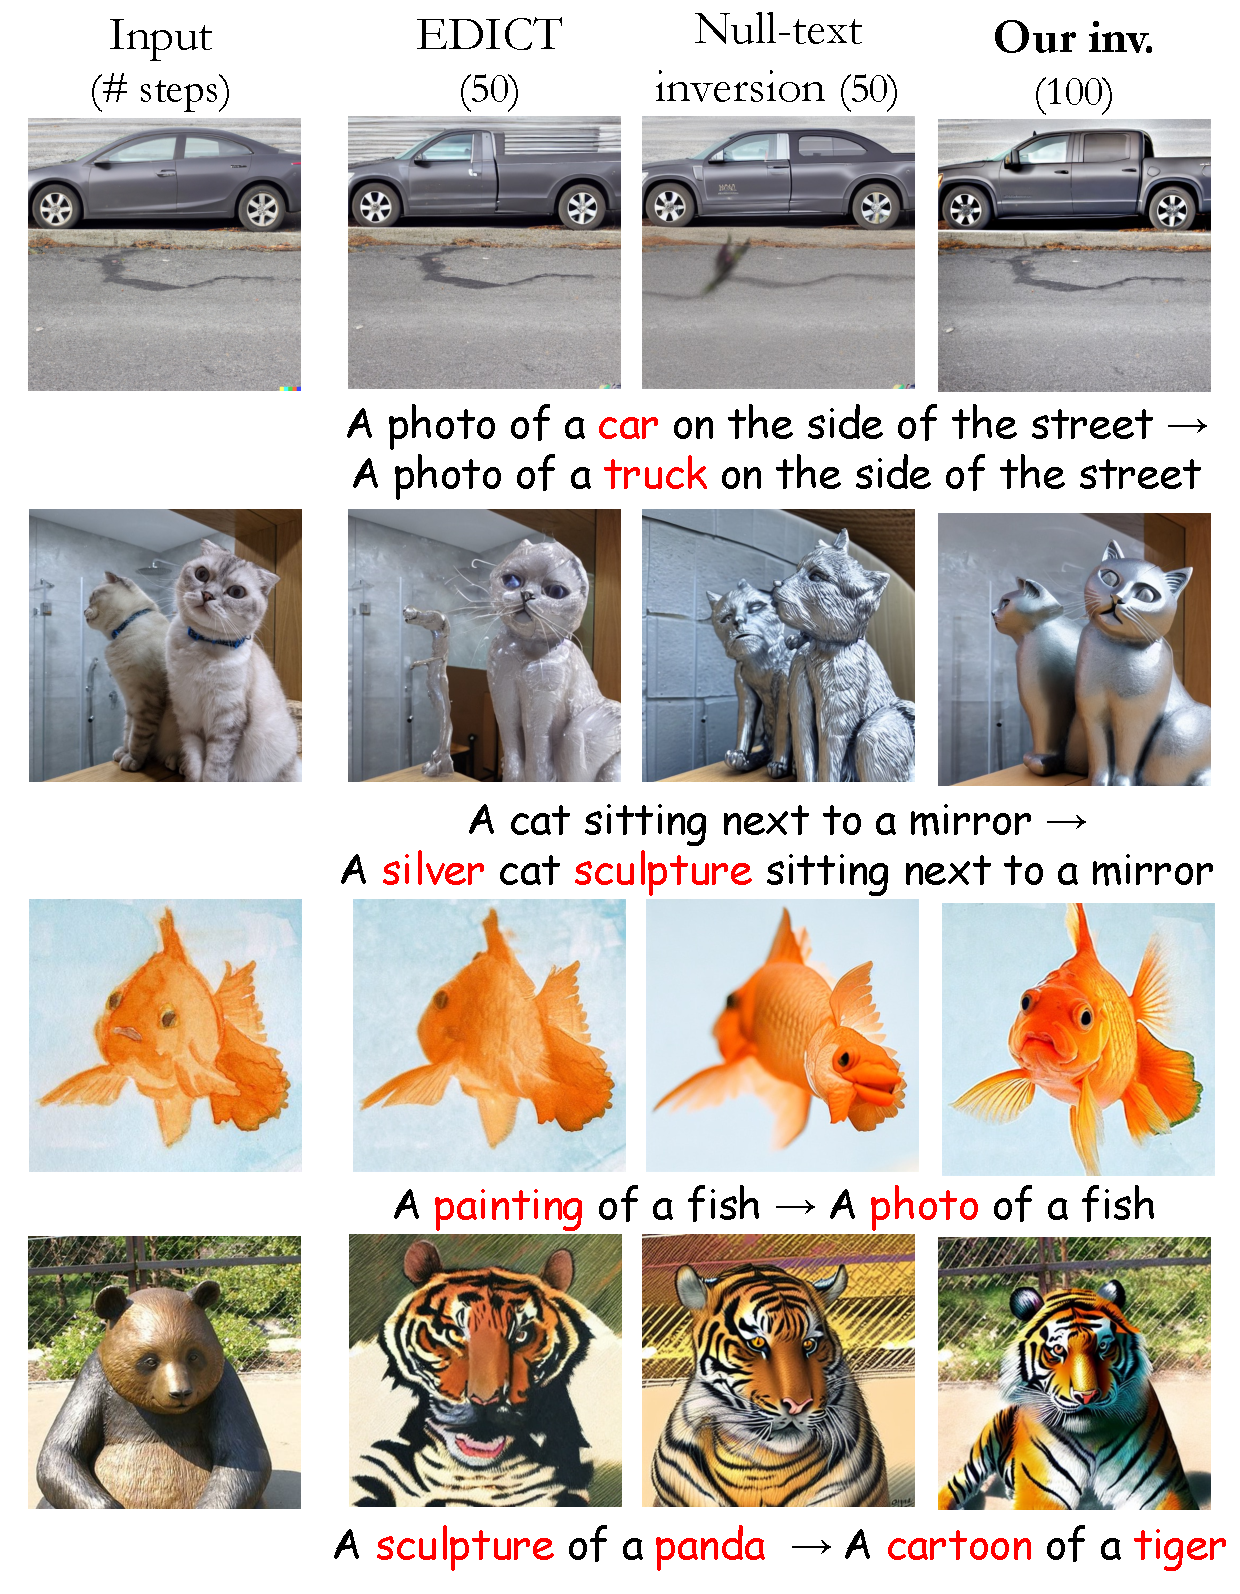
\includegraphics[width=0.7\textwidth]{ICCV23_submission/figures/comparison_EDICT_null_inversion.pdf}
% \caption{\textbf{Additional qualitative comparisons EDICT, null-text inversion and ours.}}
% \label{fig:comparison_EDICT_null_inversion}
% \end{figure*}

% \clearpage